Po zakończeniu pobierania obrazu instalatora należy nagrać go na zewnętrzny nośnik i uruchomić komputer z tego nośnika. Najlepszym rozwiązaniem jest użycie klucza USB (pendrive'a), gdyż obrazy instalacyjne Ubuntu są zbyt duże aby zmieścić się na typowych krążkach CD o pojemności 700 MB. Weź jednak pod uwagę, że nie wszystkie komputery potrafią startować z klucza USB. Jeżeli twój komputer nie pozwala na wykonanie takiej operacji, będziesz musiał użyć płyty DVD lub karty (micro)SD.
\subsubsection{System Windows, nagrywanie na pendriva}
\begin{wrapfigure}[5]{r}{0.5\textwidth}
	\vspace{-10pt}
	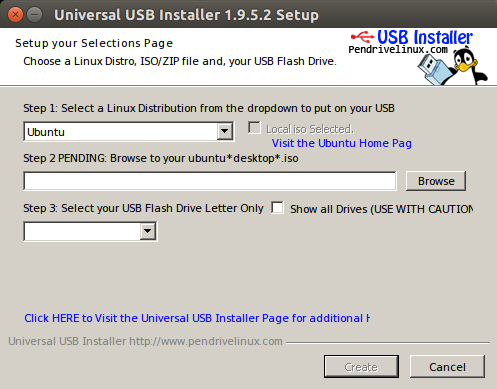
\includegraphics[width=\linewidth]{images/instalacja_nagrywanie_obrazu.png}
\end{wrapfigure}

Jeżeli chcesz użyć pendrive'a jako nośnika instalacyjnego, upewnij się, że ma on przynajmniej 1 GB pojemności (w przeciwnym wypadku instalator się tam po prostu nie zmieści). Jeżeli masz już przygotowany pendrive, wykonaj po kolei następujące kroki:
\begin{enumerate}[label=\protect\circled{\arabic*}]
\item Pobierz program \href{http://www.pendrivelinux.com/downloads/Universal-USB-Installer/Universal-USB-Installer-1.9.5.2.exe}{Universal USB Installer}.
\item Uruchom pobrany plik.
\item Zaakceptuj umowę licencyjną.
\item Podłącz do komputera pendrive, który ma użyty jako nośnik.
\item Z tej listy wybierz Ubuntu.
\item Kliknij na przycisk \textcolor{ubuntu_orange}{Browse} i wskaż pobrany wcześniej obraz instalatora Ubuntu.
\item Z tej listy wybierz podłączonego wcześniej pendrive'a.\\
\textbf{UWAGA: Wszystkie dane na nim zostaną skasowane!}
\item Kliknij przycisk \textcolor{ubuntu_orange}{Create}.
\item Poczekaj na zakończenie operacji.
\end{enumerate}
\clearpage
\subsubsection{System Windows 7 / 8, nagrywanie na płytę DVD}
%TODO zweryfikować, czy Windows 8 też to ma
\begin{wrapfigure}[10]{r}{0.5\textwidth}
	\vspace{-10pt}
	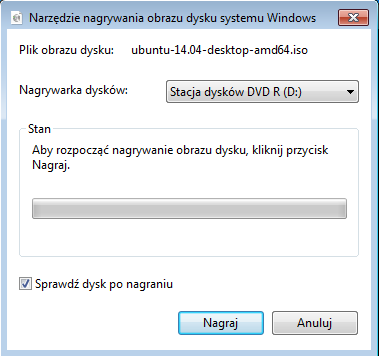
\includegraphics[width=\linewidth]{images/instalacja_nagrywanie_obrazu_DVD.png}
\end{wrapfigure}

Systemy operacyjne Windows 7 i 8 mają wbudowane narzędzie do wypalania plików .iso na płytach. Kliknij prawym przyciskiem myszy na pobrany obraz instalatora Ubuntu, wybierz opcję \textcolor{ubuntu_orange}{Otwórz w} a następnie \textcolor{ubuntu_orange}{Windows Disc Image Burner}.
%TODO jak to się po polsku nazywa?
\begin{enumerate}[label=\protect\circled{\arabic*}]
\item Z tej listy wybierz swoją nagrywarkę.
\item Włóż do wybranego napędu czystą płytę DVD.
\item Upewnij się, że zaznaczone jest pole \textcolor{ubuntu_orange}{Zweryfikuj dysk po nagraniu}
\item Kliknij na przycisk \textcolor{ubuntu_orange}{Nagraj}.
\end{enumerate}

%Pusta przestrzeń, żeby obrazi z sekcji powyżej i poniżej nie wchodziły na siebie.
\vspace{1cm}

\subsubsection{System Windows XP i inne starsze wersje, nagrywanie na płytę DVD}
\begin{wrapfigure}[10]{r}{0.5\linewidth}
	\vspace{-10pt}
	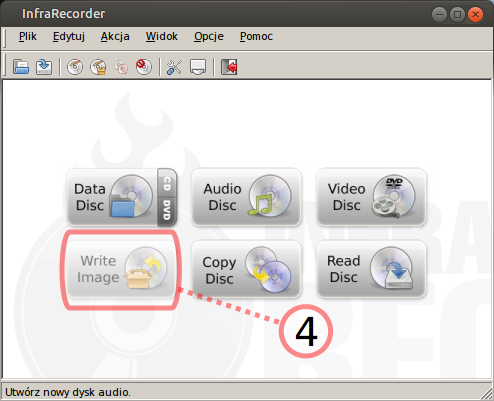
\includegraphics[width=\linewidth]{images/instalacja_nagrywanie_obrazu_DVD_winXP.png}
\end{wrapfigure}

Starsze wersje systemu Windows nie mają wbudowanej możliwości nagrywania płyt DVD. Potrzebne będzie do tego osobne narzędzie służące do wypalania płyt. Obsługa tych programów jest bardzo podobna: należy wybrać opcję Nagrywanie obrazu na płytę. Koniecznie nagrywaj z wykorzystaniem tej opcji, gdyż inne (np. Nagrywanie płyty z danymi lub Tworzenie kopi zapasowej) utworzy dysk, którego twój komputer nie będzie potem wstanie uruchomić. Dla przykładu posłużymy się programem Infra Recorder.

\begin{enumerate}[label=\protect\circled{\arabic*}]
\item Pobierz i zainstaluj program \href{http://infrarecorder.org/?page_id=5}{Infra Recorder}.
\item Uruchom zainstalowany przed momentem program.
\item Włóż czystą płytę DVD do nagrywarki.
\item W programie Infra Recorder wybierz opcję \textcolor{ubuntu_orange}{Write Image}.
\item Wybierz pobrany wcześniej obraz instalatora systemu Ubuntu.
\item Kliknij na przycisk \textcolor{ubuntu_orange}{OK}.
\end{enumerate}